\documentclass[portrait,final,a0paper,fontscale=0.277]{baposter}

\usepackage{calc}
\usepackage{graphicx}
\usepackage{amsmath}
\usepackage{amssymb}
\usepackage{relsize}
\usepackage{multirow}
\usepackage{rotating}
\usepackage{bm}
\usepackage{url}

\usepackage{graphicx}
\usepackage{multicol}
\usepackage{multirow}

\usepackage[noend]{algpseudocode}
\usepackage{algorithm}

%\usepackage{times}
%\usepackage{helvet}
%\usepackage{bookman}
\usepackage{palatino}

\newcommand{\captionfont}{\footnotesize}

\renewcommand{\familydefault}{\sfdefault}

\graphicspath{{imgs/}{../imgs/}}
\usetikzlibrary{calc}

\definecolor{cobaltBlue}{RGB}{0,51,153}
\definecolor{navyBlue}{RGB}{0,30,102}
\definecolor{lightBLue}{RGB}{37,200,255}


\begin{document}
\begin{poster}
{
  grid=false,
  eyecatcher=true,
%
  bgColorOne=white,
  headerColorOne=lightBLue,
  borderColor=navyBlue,
%
  background=plain,
  headershade=plain,
  boxshade=none,
  headerborder=closed,
  textborder=roundedsmall,
  headershape=smallrounded,
%
  headerheight=0.1\textheight
}
{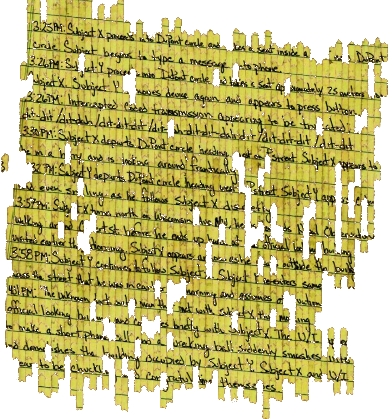
\includegraphics[height=8.5em]{images/eyecatcher.jpg} }
{\bf{\textsc{\textrm{Reconstructing shredded\vspace{0.1em} documents}}} }
{ \textsc{\textrm{Razvan Ranca}}\\[0.8em]
  \texttt{ranca.razvan@gmail.com} 
}
{
\includegraphics[height=7.5em]{images/logo.jpg} }

\headerbox{\textrm{Importance}}{name=importance,column=0,row=0}{
 	\raggedright Despite the development of techniques permitting the purely electronic storage and transmittal of sensitive documents, many such documents are still printed and eventually shredded. Traditionally, the cost of reconstructing these documents was considered prohibitive, however with the development of methods that largely automate the process this situation is changing. \vspace{0.6em} \\ It is currently unclear what level of security the paper shredder still offers.\\ \vspace{0.5em}

\begin{minipage}{0.5\linewidth}
  \center
  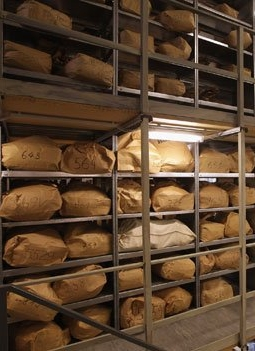
\includegraphics[height=8em]{images/stasiSmall.jpg}
\end{minipage}
\begin{minipage}{0.47\linewidth}
  \center
  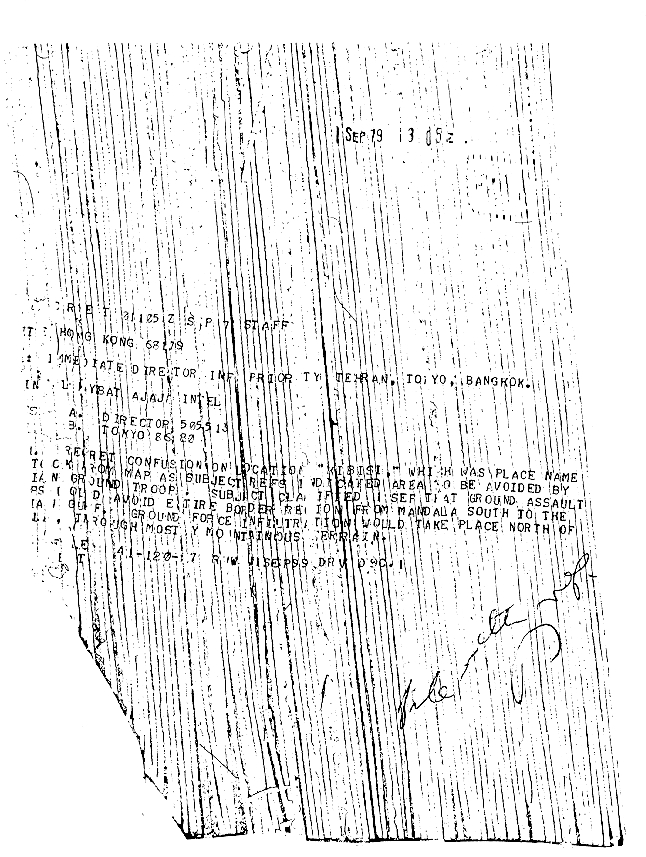
\includegraphics[height=8em]{images/iran.jpg}
\end{minipage}
\begin{minipage}{0.51\linewidth}
  \center
  \smaller
   A few of the 16,000 bags holding the shredded archives of the East German secret police
\end{minipage}
\begin{minipage}{0.46\linewidth}
  \center
  \smaller
  A shredded document reconstructed during the Iran hostage crisis
\end{minipage}
}

\headerbox{\textrm{Probabilistic Score}}{name=probScore,column=0,below=importance}{
\algrenewcommand\algorithmicindent{0.8em}
\begin{algorithmic}
\Procedure {ProbScore}{$Et$}
  \State {Initialize $pr$} 
  \ForAll{$Ex \in Edges$} 
    \ForAll {$pixel \in Ex$}
      \State $pr_{Ex} \gets pr_{Ex} * \Pr(pixel|Neighbors_{Et})$ 
    \EndFor
  \EndFor
  \State {Normalize $pr$} 
  \State {Assert: $ \sum_{Ex \in Edges} pr_{Ex}=1$} 
  \State \textbf{return} $\max pr$, $\arg\max pr$
\EndProcedure
\end{algorithmic}
\begin{minipage}{0.98\linewidth}
\vspace{0.2em} \raggedright {ProbScore returns the most likely match for the input edge $Et$, and the probability of that match being correct.}
\end{minipage}
}

\headerbox{\textrm{Probabilistic Score - Evaluation}}{name=results,column=1,span=2,row=0}{

    \begin{minipage}[t]{0.48\linewidth}
       	\raggedright The probabilistic score function is evaluated against the best previously published cost function \cite{P1,P2}. The comparison looks at both noisy and noise-less documents. \vspace{0.5em} \\ ProbScore outperforms the Gaussian cost on three out of the four instances.
    \end{minipage}
    \fbox{
    \begin{minipage}[t]{0.48\linewidth}
        \centering
        \begin{minipage}[t]{0.48\linewidth}
                \centering
                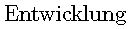
\includegraphics[width=\textwidth]{EntOrig}
        \end{minipage}
        \begin{minipage}[t]{0.48\linewidth}
                \centering
                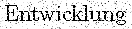
\includegraphics[width=\textwidth]{EntNoise}
        \end{minipage}
        \begin{minipage}[t]{0.48\linewidth}
                \centering
                \smaller Original image
        \end{minipage}
        \begin{minipage}[t]{0.48\linewidth}
                \centering
                \smaller 10\% of pixels are randomly flipped
        \end{minipage}
        \begin{minipage}[t]{0.48\linewidth}
                \centering
                
\includegraphics[width=\textwidth]{EntDown}
        \end{minipage}
        \begin{minipage}[t]{0.48\linewidth}
                \centering
                
\includegraphics[width=\textwidth]{EntSpread}
        \end{minipage}
        \begin{minipage}[t]{0.48\linewidth}
                \centering
                \smaller Downsampled by a factor of 1.5
        \end{minipage}
        \begin{minipage}[t]{0.48\linewidth}
                \centering
                \smaller Pixels shuffled with neighbours
        \end{minipage}
    \end{minipage}
    }

    \begin{minipage}[t]{0.98\linewidth}
        \centering
        \begin{minipage}[t]{0.48\linewidth}
                \centering
                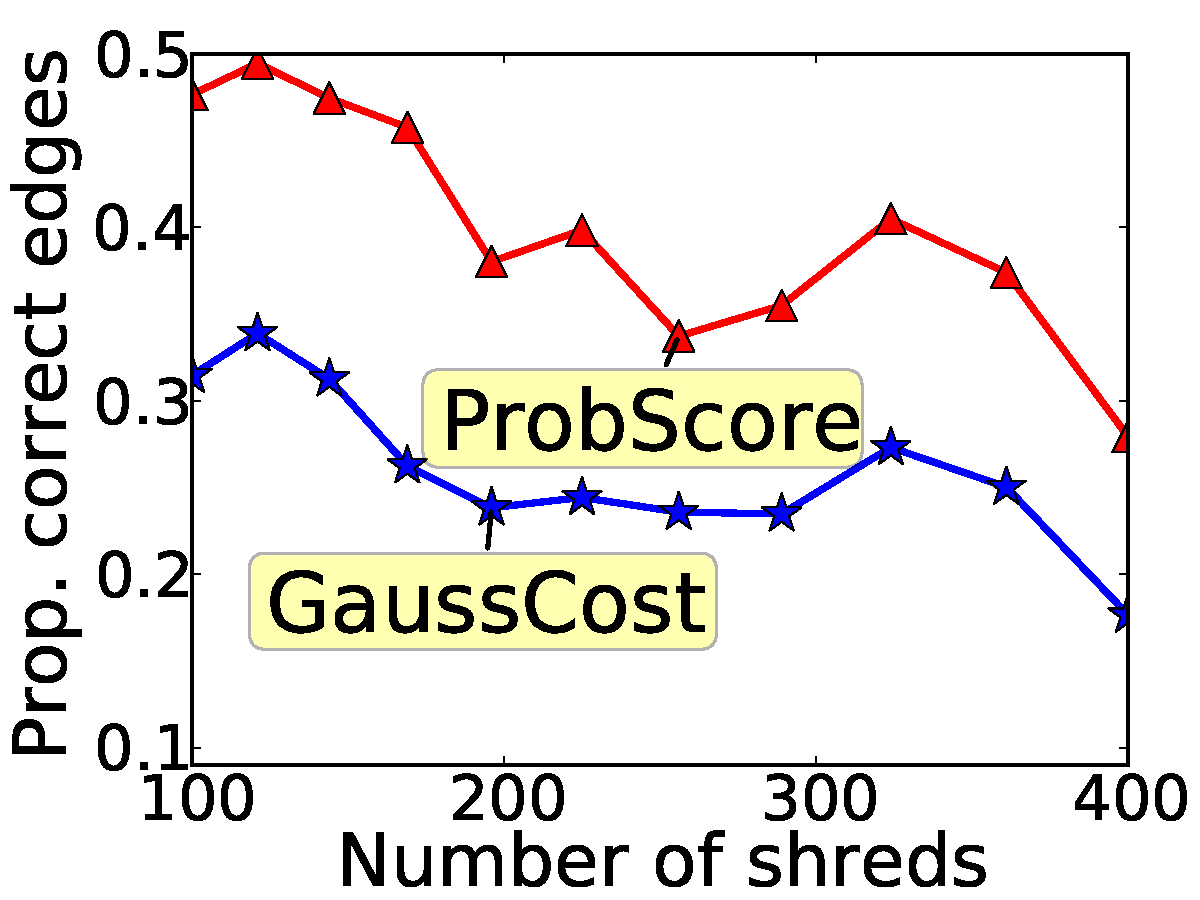
\includegraphics[width=\textwidth]{origComp}
        \end{minipage}
        \begin{minipage}[t]{0.48\linewidth}
                \centering
                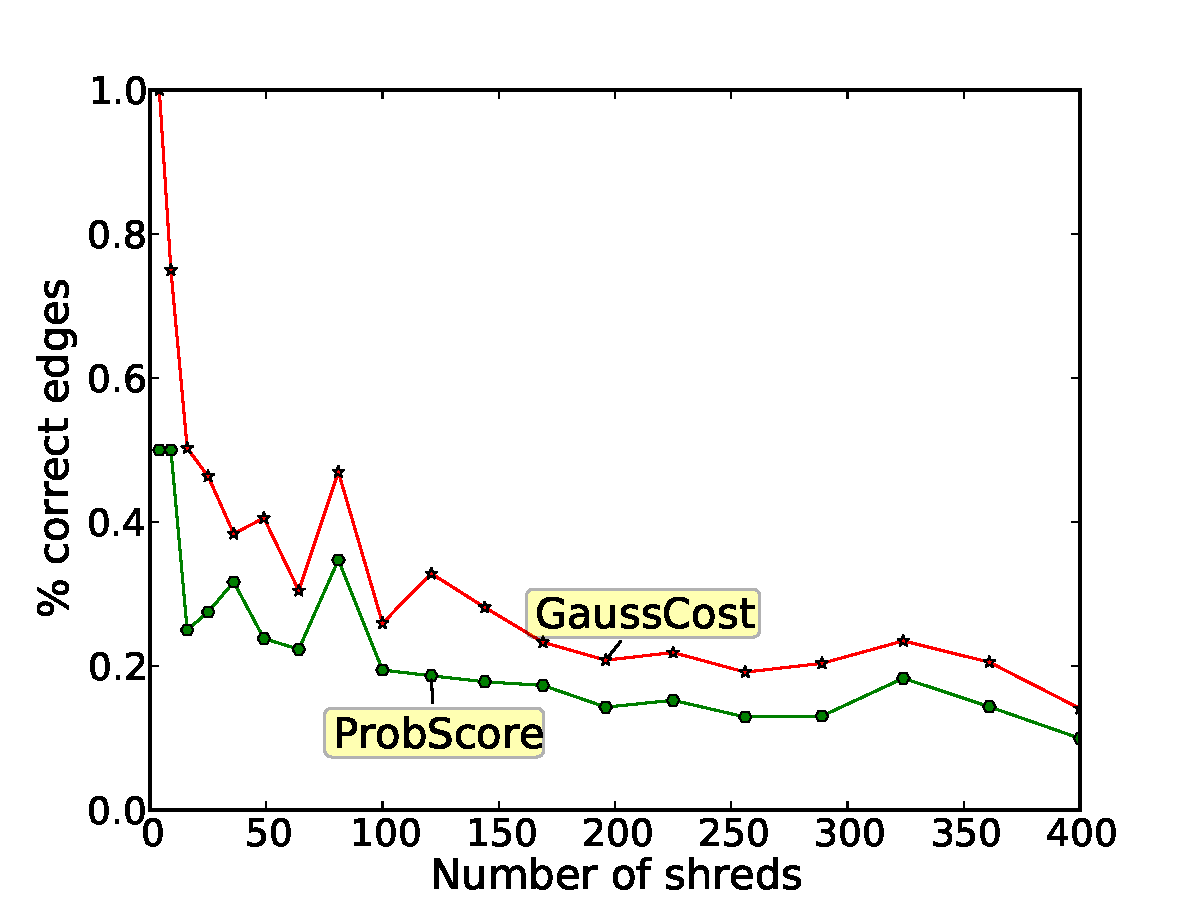
\includegraphics[width=\textwidth]{noise}
        \end{minipage}
        \begin{minipage}[t]{0.48\linewidth}
                \centering
                \smaller Original image
        \end{minipage}
        \begin{minipage}[t]{0.48\linewidth}
                \centering
                \smaller 10\% of pixels are randomly flipped
        \end{minipage}
        \begin{minipage}[t]{0.48\linewidth}
                \centering
                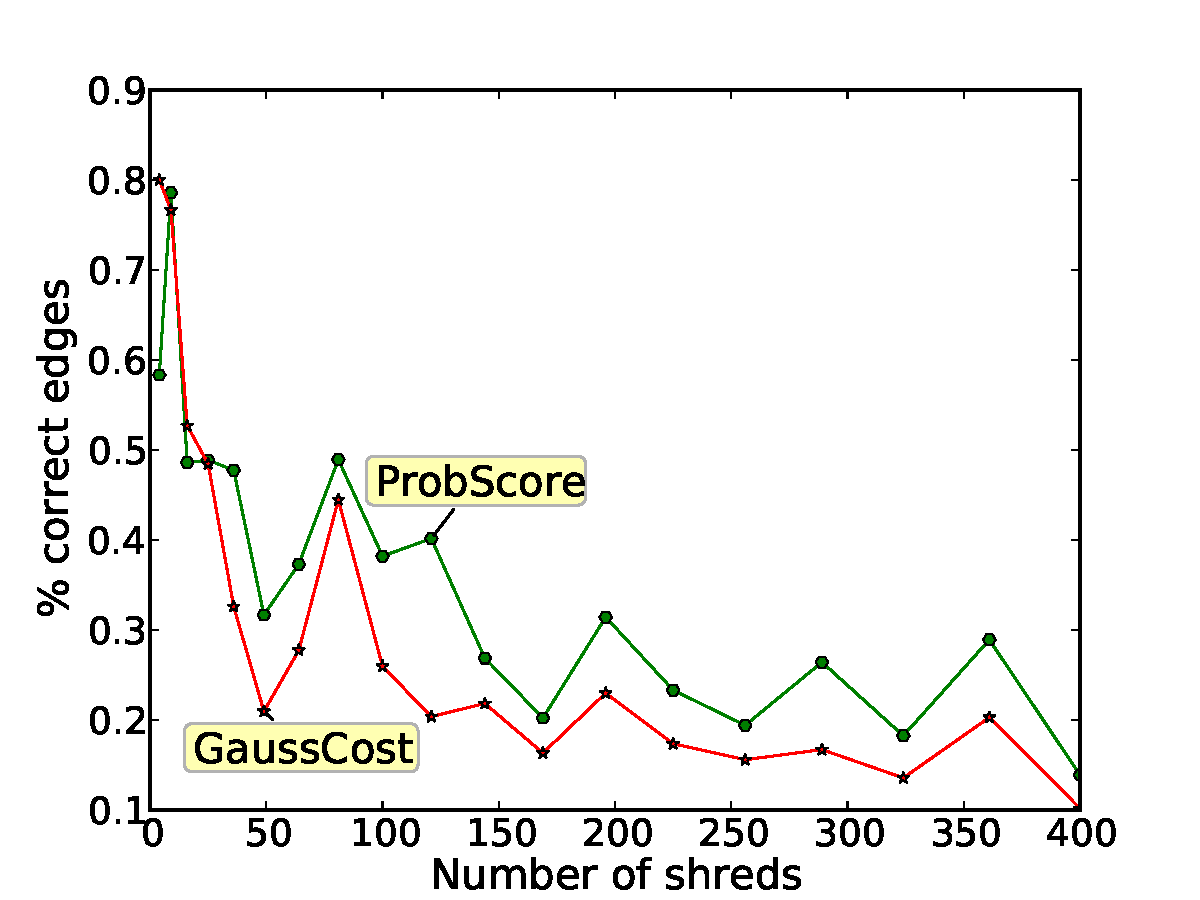
\includegraphics[width=\textwidth]{downsample}
        \end{minipage}
        \begin{minipage}[t]{0.48\linewidth}
                \centering
                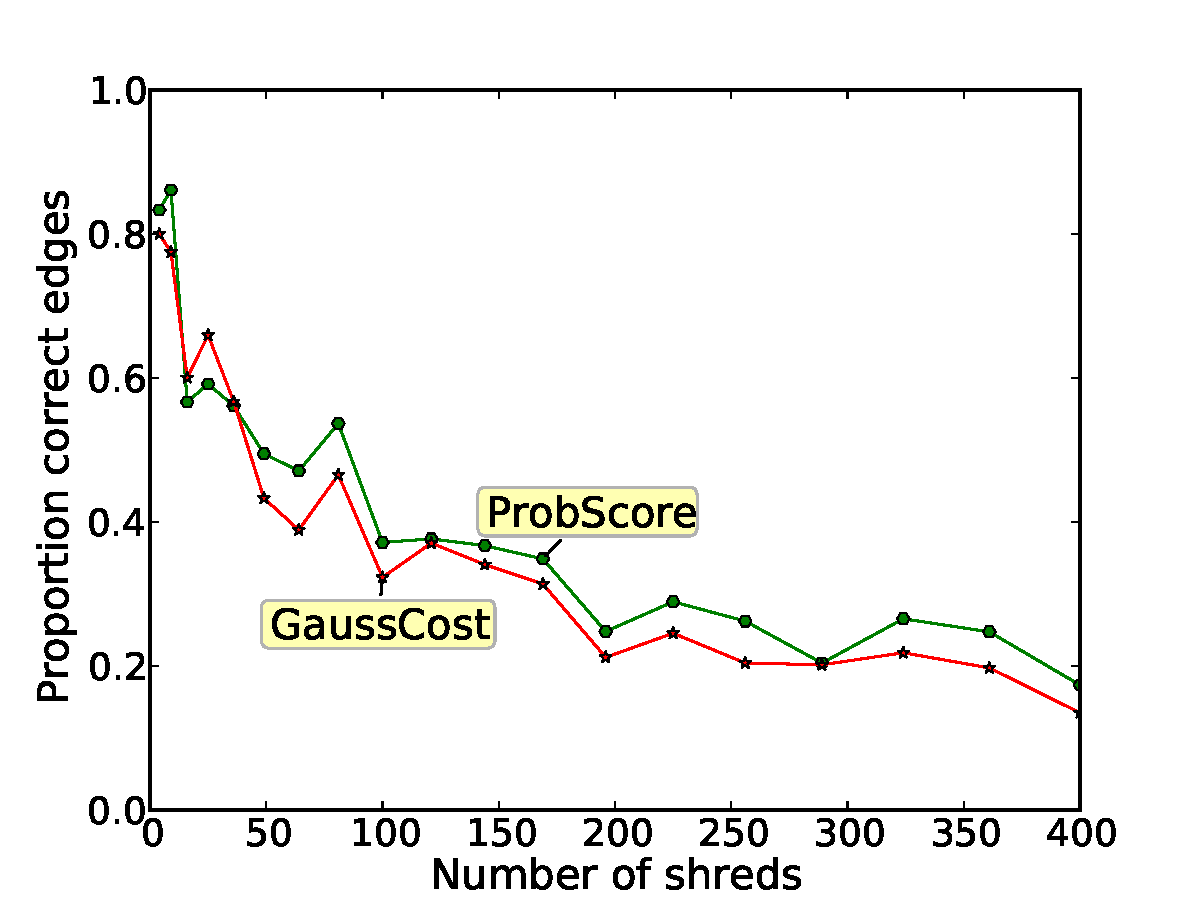
\includegraphics[width=\textwidth]{shuffle}
        \end{minipage}
        \begin{minipage}[t]{0.48\linewidth}
                \centering
                \smaller Downsampled by a factor of 1.5
        \end{minipage}
        \begin{minipage}[t]{0.48\linewidth}
                \centering
                \smaller Pixels randomly shuffled with neighbours
        \end{minipage}
    \end{minipage}
}

\headerbox{\textrm{Row detection}}{name=search,column=1,below=results}{
        \begin{minipage}[t]{0.98\linewidth}
                \centering
                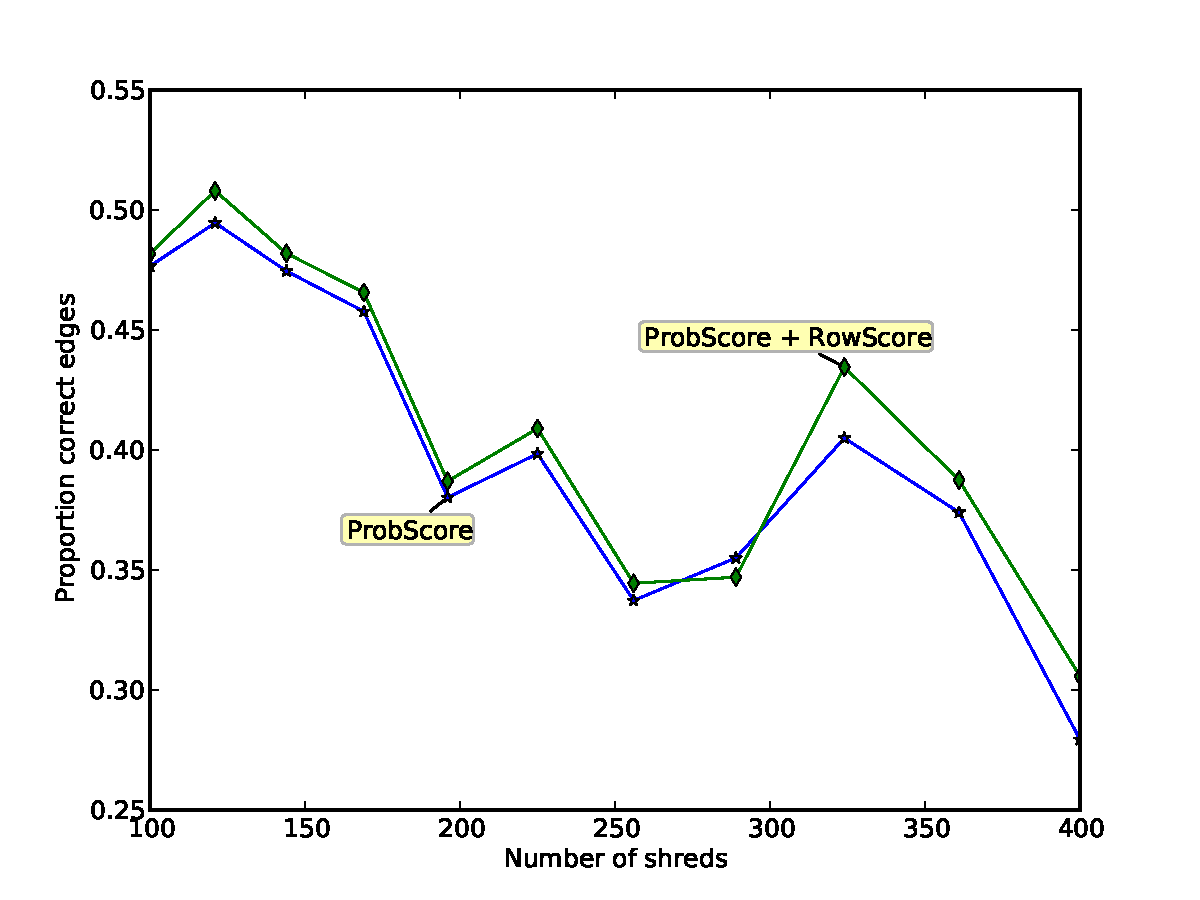
\includegraphics[width=\textwidth]{rowScore.pdf}
        \end{minipage}
        \begin{minipage}[t]{0.98\linewidth}
                \centering
                \smaller Simple Gaussian model on distance between matching rows improves accuracy slightly
        \end{minipage}
        \begin{minipage}[t]{0.98\linewidth}
                \centering
                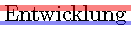
\includegraphics[width=0.68\textwidth]{EntRow.png}
        \end{minipage}
        \begin{minipage}[c]{0.98\linewidth}
                \centering
                \smaller Orientation detection can be performed by counting the pixels in the upper and lower regions and predicting that more black pixels will be on top
        \end{minipage}
        \begin{minipage}[t]{0.98\linewidth}
                \centering \vspace{0.3em}
                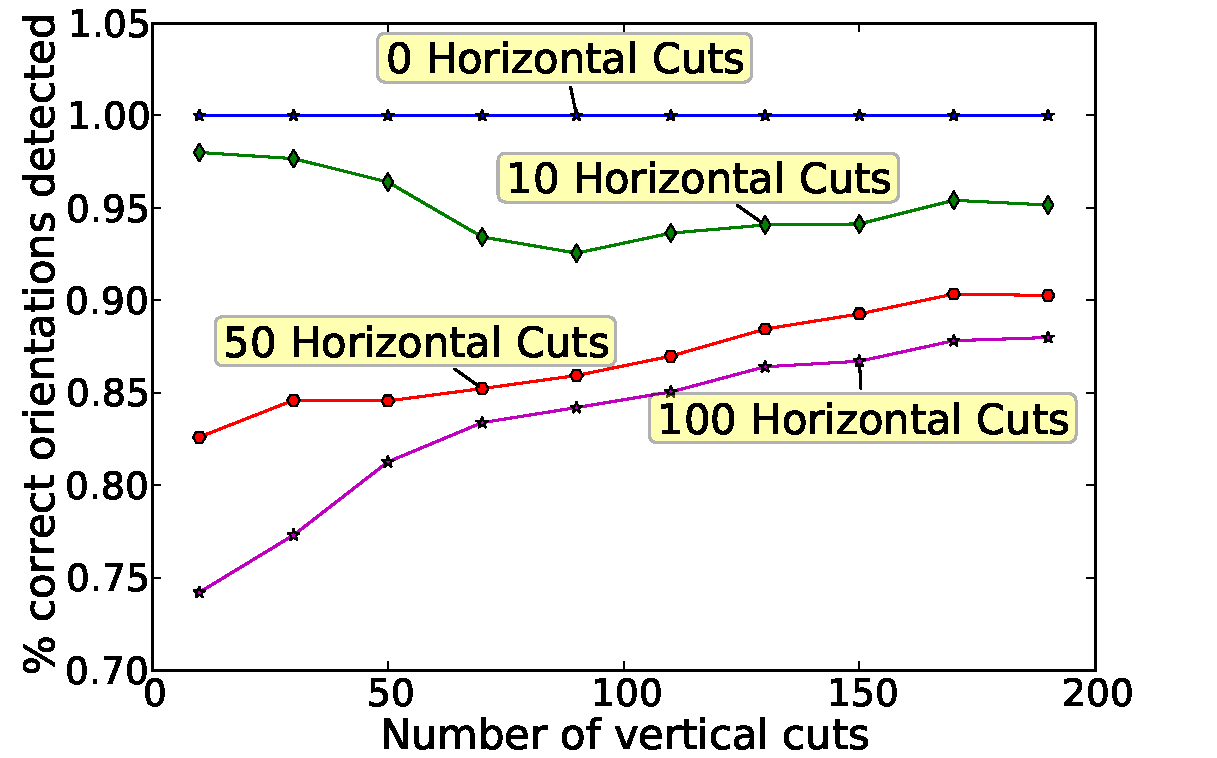
\includegraphics[width=\textwidth]{orientation.pdf}
        \end{minipage}

}

\headerbox{\textrm{Kruskal-inspired Search}}{name=search,column=0,below=probScore}{
    \begin{minipage}[t]{0.98\linewidth}
        \centering
        \begin{minipage}[c]{0.37\linewidth}
                \centering
                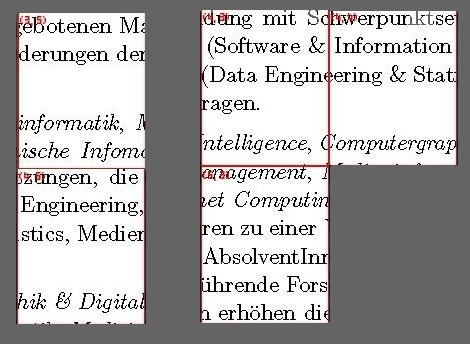
\includegraphics[width=\textwidth]{kruskalS1Grey}
        \end{minipage}
        \begin{minipage}[c]{0.61\linewidth}
                \centering
                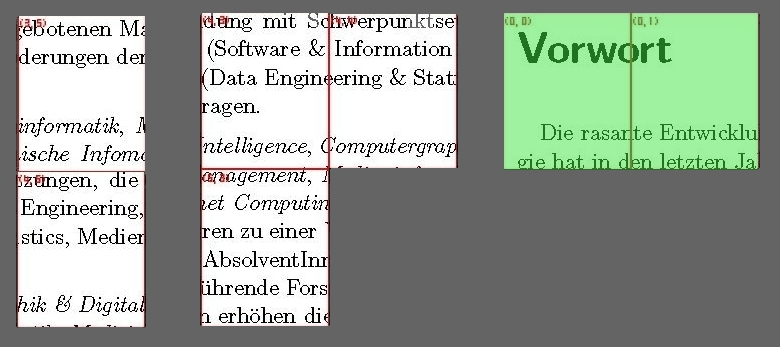
\includegraphics[width=\textwidth]{kruskalS2Grey}
        \end{minipage}

        \begin{minipage}[t]{0.37\linewidth}
                \centering
                \smaller Initially, two clusters present
        \end{minipage}
        \begin{minipage}[t]{0.61\linewidth}
                \centering
                \smaller A new cluster can be formed
        \end{minipage}

        \begin{minipage}[c]{0.56\linewidth}
                \centering
                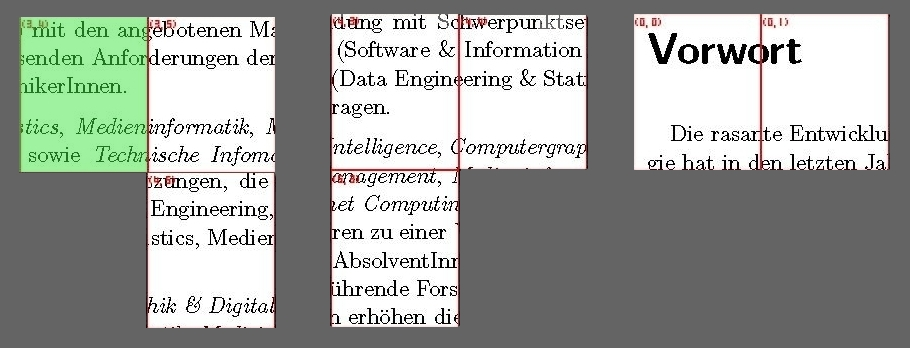
\includegraphics[width=\textwidth]{kruskalS3Grey}
        \end{minipage}
        \begin{minipage}[c]{0.42\linewidth}
                \centering
                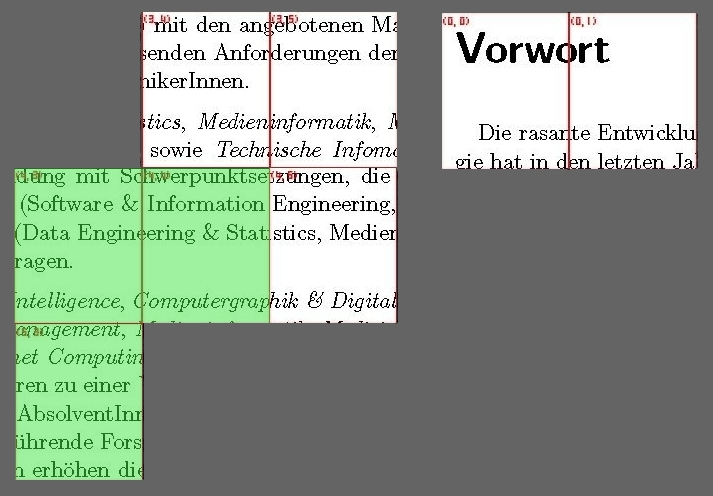
\includegraphics[width=\textwidth]{kruskalS4Grey}
        \end{minipage}

        \begin{minipage}[t]{0.56\linewidth}
                \centering
                \smaller An existing cluster can be enlarged
        \end{minipage}
        \begin{minipage}[t]{0.42\linewidth}
                \centering
                \smaller Two existing clusters can be merged
        \end{minipage}
    \end{minipage}

    \begin{minipage}[t]{0.98\linewidth}
    \vspace{1em}
     	\raggedright The "Kruskal" heuristic is based on the "ReconstructShreds" method presented in \cite{P1}. Analogous to the minimum spanning tree "Kruskal's Algorithm", this method tries to greedily unite the two best matching edges at every step. \\ The main difference from the basic algorithm is that the shreds need to have a specific position in 2D space and therefore uniting two pieces can cause an overlap. Any such overlap would lead to an illegal solution and so must be prevented.
    \end{minipage}
}

\headerbox{\textrm{Results}}{name=shreddercomp,column=2,below=results}{
  \begin{minipage}[t]{0.4\linewidth}
    \begin{minipage}[t]{\linewidth}
      \centering
      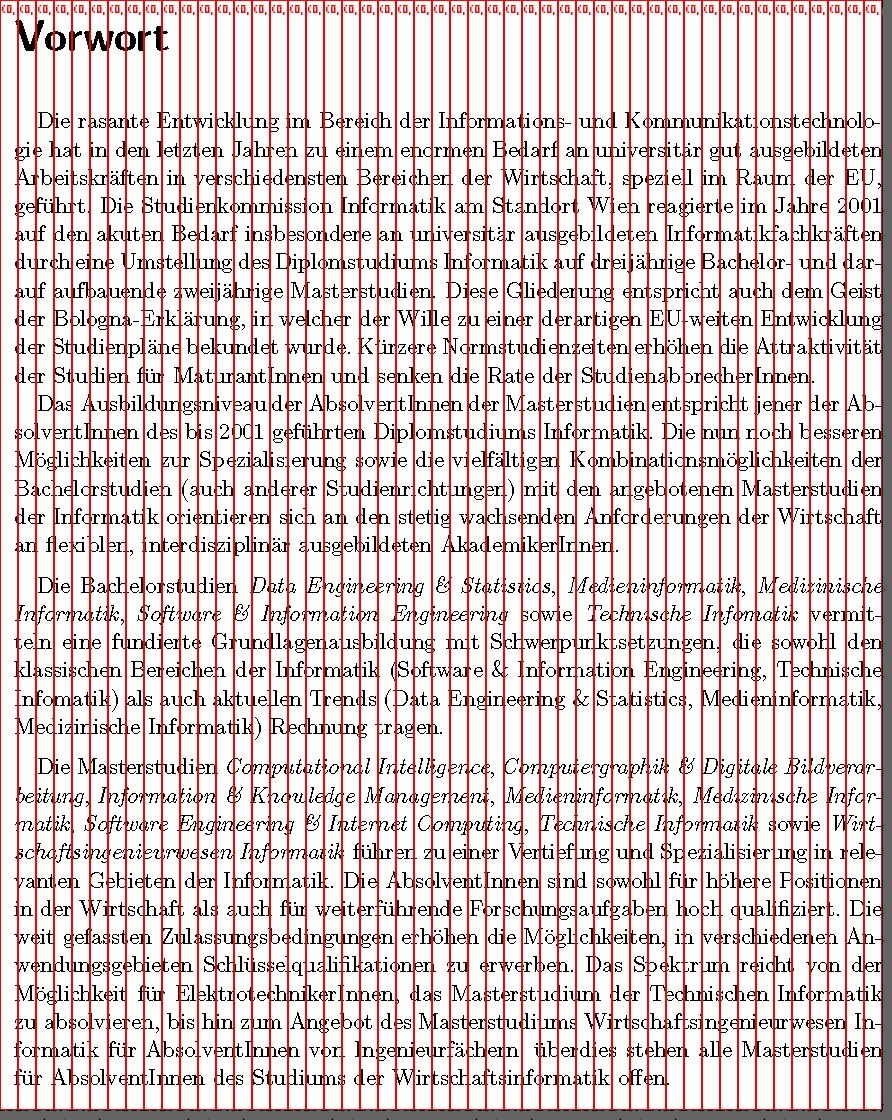
\includegraphics[width=\textwidth]{ss49Grey}
      \smaller Strip shredder
    \end{minipage}

    \begin{minipage}[t]{\linewidth}
      \centering
      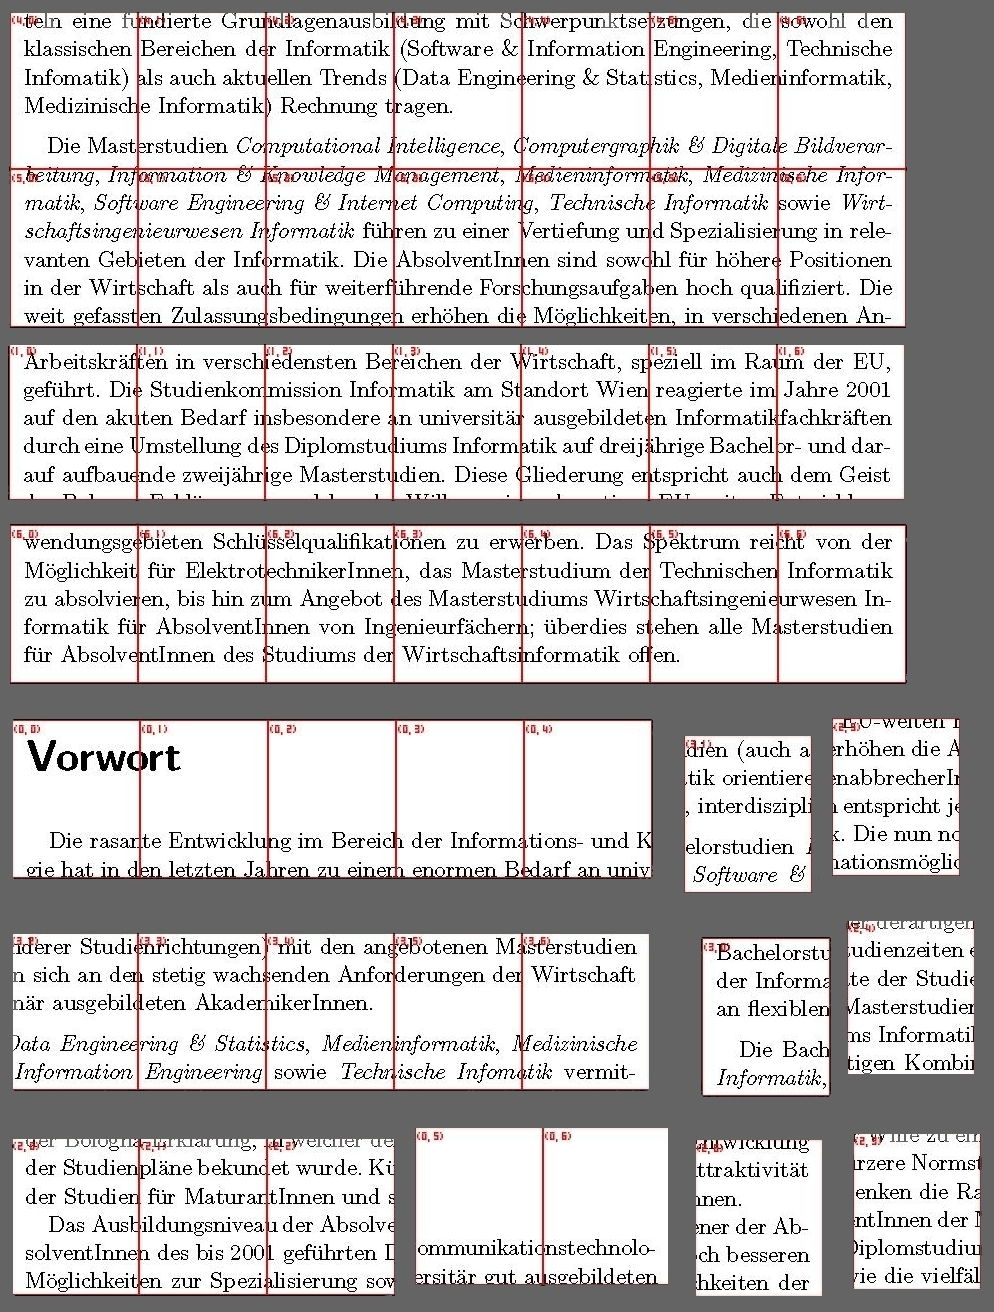
\includegraphics[width=\textwidth]{cc49Grey}
      \smaller Cross-cut shredder
    \end{minipage}
  \end{minipage}
  \begin{minipage}[c]{0.57\linewidth}
     	\raggedright Both images are of documents cut into 49 shreds. While the strip shredded variant is perfectly reconstructed, only certain sections of the cross-cut document can be recovered with any certainty. \vspace{1em} \\ Even if the total number of shreds is the same, the cross-cut case is \emph{much} harder to solve.
  \end{minipage}
}

\headerbox{\textrm{References}}{name=references,column=2,below=shreddercomp}{
  \smaller
  \bibliographystyle{ieee}
  \renewcommand{\section}[2]{\vskip 0.05em}
    \begin{thebibliography}{1}\itemsep=-0.01em
    \setlength{\baselineskip}{0.4em}
    \bibitem{P1}
       Sleit, A., Massad, Y. and Musaddaq M.
      \newblock An alternative clustering approach for reconstructing cross cut shredded text documents
      \newblock In {\em Telecommunication Systems '11}
    \bibitem{P2}
       Prandtstetter, M. and Raidl, G.
      \newblock Combining Forces to Reconstruct Strip Shredded Text Documents
      \newblock In {\em Hybrid metaheuristics '08}
    \end{thebibliography}
}

\end{poster}
\end{document}
